\section{Formulación del problema}
El objetivo de este proyecto es el diseño y análisis de un convertidor boost para cargadores de baterías
utilizados en vehículos eléctricos. Este convertidor es fundamental para transformar la corriente
alterna (AC) proveniente de la red eléctrica en corriente continua (DC) para alimentar las baterías del
vehículo. Además, se busca optimizar tanto el factor de potencia como reducir la distorsión armónica
de corriente en el proceso de carga.

El sistema propuesto incluye los componentes clave del convertidor como la bobina (L), el
condensador (C), el diodo (D) y el MOSFET (Q). El MOSFET (Q) es un transistor de efecto de
campo de óxido metálico, el cual actúa como interruptor de alta velocidad en el circuito. Su función
principal es controlar la energía almacenada en el inductor (L), conmutando a frecuencias altas para
generar el aumento de voltaje necesario en el proceso de carga de las baterías. A su vez, el modelo
contempla el comportamiento de la batería, representada por una resistencia interna (\(R_{bat}\)) y una
fuente de voltaje \(V_{bat}\), lo que permite analizar el impacto de estos elementos en la eficiencia del
sistema.

En este modelo, se asume que el sistema opera en un régimen lineal, lo cual facilita el análisis
matemático. Sin embargo, se reconoce que este supuesto no considera posibles efectos no lineales en
condiciones extremas, los cuales podrían ser un área de estudio adicional en futuros trabajos.

El modelo está representado por las siguientes ecuaciones de pequeña señal:

% === FIGURA 1 ===
\begin{figure}[h]
    \centering
    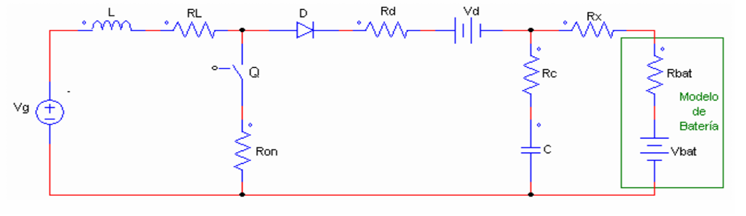
\includegraphics[width=0.8\textwidth]{1.png} % Reemplazar con ruta real
    \caption{Convertidor Boost con pérdidas en los elementos y modelo de batería.}
    \label{fig:convertidor}
\end{figure}

\[V_L(s) = V_G(s) - I_L(s) \cdot R_{eq} - V_d \cdot D' - V_0 \cdot D'\]
\[I_C(s) = \frac{[V_0(s) - V_{bat}]}{R_0} + I_L(s) \cdot D'\]

Donde:
\begin{itemize}
    \item \( R_0 + R_{x'} \cdot R_{eq} = R_L + R_{on} \cdot D + R_d \cdot D' \), \( D \) es el ciclo de la señal PWM que controla el interruptor \( Q \) y \( D' = 1 - D \)
    \item \(s\) → Es la variable de Laplace utilizada en las ecuaciones de modelo de pequeña señal
    \item \(V_L(s)\) → Es el voltaje de la inductancia.
    \item \(V_G(s)\) → Es la tensión de entrada de la red eléctrica.
    \item \(I_L(s)\) → Es la corriente a través de la bobina.
    \item \(I_C(s)\) → Es la corriente que fluye a través del convertidor.
    \item \(V_d\) → Es el voltaje del diodo.
    \item \(D'\) → Es el ciclo útil del interruptor MOSFET.
    \item Donde \(D'\) representa la señal PWM que controla el interruptor \(Q\) y \(D' = 1 - D\), donde \(D\) es el ciclo de la señal PWM
    \item \(V_0(s)\) → Es la tensión de salida.
    \item \(R_{eq}\) → Es la resistencia equivalente de la inductancia.
\end{itemize}
\newpage

% === TEXTO ORIGINAL CORREGIDO ===
Para el modelo de gran señal

% === FIGURA 2 ===
\begin{figure}[H] % H mayúscula fuerza posición exacta
    \centering
    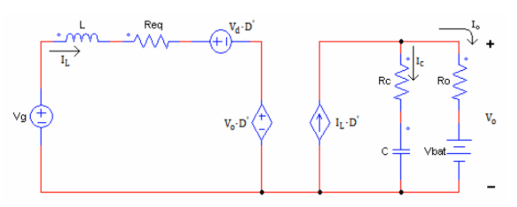
\includegraphics[width=0.8\textwidth]{3.png}
    \caption{Circuito equivalente de gran señal del convertidor boost.}
\end{figure}
Al introducir perturbaciones al modelo de gran señal, obtenemos un modelo dinámico de señal pequeña.

Modelo de pequeña señal:

% === FIGURA 3 ===
\begin{figure}[h]
    \centering
    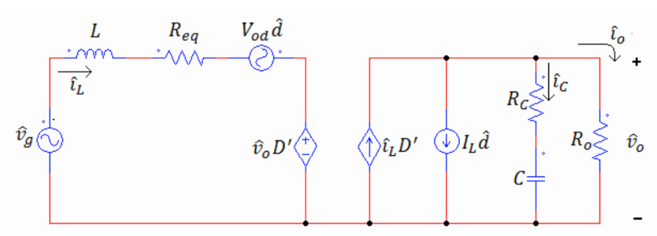
\includegraphics[width=0.8\textwidth]{2.png} % Reemplazar con ruta real
    \caption{Modelo de pequeña señal del convertidor boost}
    \label{fig:pequena_senal}
\end{figure}

\[0 = \hat{V}_g - \hat{i}_L(sL + R_{eq}) + V_{od} \hat{d} = \hat{V}_0 D'\]
\[0 = \frac{\hat{V}_0}{Z_c} + \frac{\hat{V}_0}{R_0} - \hat{i}_L D' + I_L \hat{d}\]

Donde:
\begin{itemize}
    \item \(V_{od} = V_0 + V_d\)
    \item \(Z_c = R_c + \frac{1}{sC}\)
\end{itemize}

Estas ecuaciones son fundamentales para calcular la eficiencia del sistema, ya que permiten identificar
el comportamiento de las corrientes y tensiones involucradas.

\subsection*{Función de transferencia de convertidor boost:}
A partir del modelo de pequeña señal y la utilización de métodos algebraicos para las ecuaciones
anteriores, se obtendrán las siguientes ecuaciones de transferencia. Estas expresiones permiten
establecer la relación entre la corriente en la bobina \(i_L\), la tensión de salida \(v_0\), la corriente de salida \(i_0\)
y el ciclo útil \(d\), las cuales son fundamentales para el diseño de los controladores (Paipa et al., 2020).

\begin{align*}
    G_{i_{l-} d}(s)   & = \frac{\hat{i}_L}{\hat{d}} = \frac{sC(R_0 + R_c)V_{od} + R_0 I_L D'}{s^2 C(R_0 + R_c)L + sL + C(R_0 + R_c)R_{eq} + R_0 R_c C D'^2 + R_0 D'^2 + R_{eq}}                                                                                \\
    G_{v_{0-} d}(s)   & = \frac{\hat{v}_0}{\hat{d}} = \frac{s^2(-R_0 R_c C I_L L) + s( R_c R_0 C V_{od} D' - R_0 I_L L - R_c R_0  C R_{eq} I_L) + R_0(V_{od} D' - R_{eq} I_L)}{s^2 C(R_0 + R_c)L + sL + C(R_0 + R_c)R_{eq} + R_0 R_c C D'2 + R_0 D'2}          \\
    G_{v_{0-^i L}}(s) & = \frac{\hat{v}_0}{\hat{i}_L} = \frac{s^2(-R_0 R_c C I_L L) + s( R_c R_0 C V_{od} D' - R_0 I_L L - R_c R_0  C R_{eq} I_L) + R_0(V_{od} D' - R_{eq} I_L)}{s(C(R_0 + R_c)V_{od} +  R_c R_0 CI_LD') + R_0I_LD' + V_{od}}                  \\
    G_{v_{0-^d}}(s)   & = \frac{\hat{v}_0}{\hat{d}} = \frac{s^2(-R_c R_0 C L_L L) + s( R_c R_0 C V_{od} D' - R_0 I_L L - R_c R_0  C R_{eq} I_L) + R_0(V_{od} D' - R_{eq} I_L)}{s^2 C(R_0 + R_c)LR_0 + s(L + C(R_0 + R_c)R_{eq} + R_c R_0D'2)R_0 + R_0 D'2 R_0} \\
\end{align*}

\section*{Parámetros relevantes para el estudio:}
Este modelo es una interpretación grupal basada en el modelo propuesto en estudios previos,
que fue recuperado de un paper. El principio subyacente es el mismo: identificar el recorrido
de la corriente a través del tiempo en un circuito que alimenta la batería de un automóvil
eléctrico.

La delimitación y reducción del circuito a una malla proporciona una representación
aproximada de la dinámica que sigue la corriente en el sistema, considerando la proporción de
la energía transferida. Esto permite realizar un análisis del comportamiento del cargador de la
batería, lo cual es crucial para evaluar cómo se comporta el sistema de carga en diferentes
condiciones.

El modelo resultante tendrá valores aproximados que están alineados con los requerimientos
específicos que un vehículo eléctrico de estas características necesita para funcionar
correctamente. Al plantear la ecuación diferencial propuesta, se siguieron los siguientes
métodos analíticos resolutivos, los cuales servirán como herramienta fundamental para el
despeje y posterior descripción del comportamiento de la corriente que alimenta la batería del
vehículo eléctrico.

Y estos son los parámetros clave de los componentes que influyen directamente en el diseño y
rendimiento del sistema de carga, los cuales se incorporan en el modelo del convertidor boost
para optimizar la eficiencia y estabilidad del proceso.

\begin{enumerate}
    \item \textbf{Resistor (Resistencia)}
          \begin{itemize}
              \item \textbf{Función:} Limita el flujo de corriente en un circuito.
              \item \textbf{Características:} Convierte energía eléctrica en calor mediante la resistencia. Su valor se mide en ohmios (\(\Omega\)).
              \item \textbf{Uso Común:} Control de corriente, divisores de tensión, y protección de componentes.
          \end{itemize}

    \item \textbf{Capacitor (Condensador)}
          \begin{itemize}
              \item \textbf{Función:} Almacena y libera energía eléctrica en forma de campo eléctrico.
              \item \textbf{Características:} Puede almacenar carga eléctrica temporalmente y su capacidad se mide en faradios (\(F\)).
              \item \textbf{Uso Común:} Filtrado de señales, estabilización de voltaje, y almacenamiento de energía.
          \end{itemize}

    \item \textbf{Bobina (Inductor)}
          \begin{itemize}
              \item \textbf{Función:} Almacena energía en un campo magnético cuando circula corriente a través de ella.
              \item \textbf{Características:} Resiste cambios en la corriente y su inductancia se mide en henrios (\(H\)).
              \item \textbf{Uso Común:} Filtrado de señales, almacenamiento de energía en convertidores, y en transformadores.
          \end{itemize}

    \item \textbf{Diodo}
          \begin{itemize}
              \item \textbf{Función:} Permite el flujo de corriente en una sola dirección.
              \item \textbf{Características:} Tiene una baja resistencia en la dirección de conducción (polarización directa) y una alta resistencia en la dirección opuesta (polarización inversa).
              \item \textbf{Uso Común:} Rectificación de corriente AC a DC, protección contra polaridad inversa, y regulación de voltaje.
          \end{itemize}
\end{enumerate}